
%% bare_conf.tex
%% V1.3
%% 2007/01/11
%% by Michael Shell
%% See:
%% http://www.michaelshell.org/
%% for current contact information.
%%
%% This is a skeleton file demonstrating the use of IEEEtran.cls
%% (requires IEEEtran.cls version 1.7 or later) with an IEEE conference paper.
%%
%% Support sites:
%% http://www.michaelshell.org/tex/ieeetran/
%% http://www.ctan.org/tex-archive/macros/latex/contrib/IEEEtran/
%% and
%% http://www.ieee.org/

%%*************************************************************************
%% Legal Notice:
%% This code is offered as-is without any warranty either expressed or
%% implied; without even the implied warranty of MERCHANTABILITY or
%% FITNESS FOR A PARTICULAR PURPOSE! 
%% User assumes all risk.
%% In no event shall IEEE or any contributor to this code be liable for
%% any damages or losses, including, but not limited to, incidental,
%% consequential, or any other damages, resulting from the use or misuse
%% of any information contained here.
%%
%% All comments are the opinions of their respective authors and are not
%% necessarily endorsed by the IEEE.
%%
%% This work is distributed under the LaTeX Project Public License (LPPL)
%% ( http://www.latex-project.org/ ) version 1.3, and may be freely used,
%% distributed and modified. A copy of the LPPL, version 1.3, is included
%% in the base LaTeX documentation of all distributions of LaTeX released
%% 2003/12/01 or later.
%% Retain all contribution notices and credits.
%% ** Modified files should be clearly indicated as such, including  **
%% ** renaming them and changing author support contact information. **
%%
%% File list of work: IEEEtran.cls, IEEEtran_HOWTO.pdf, bare_adv.tex,
%%                    bare_conf.tex, bare_jrnl.tex, bare_jrnl_compsoc.tex
%%*************************************************************************

% *** Authors should verify (and, if needed, correct) their LaTeX system  ***
% *** with the testflow diagnostic prior to trusting their LaTeX platform ***
% *** with production work. IEEE's font choices can trigger bugs that do  ***
% *** not appear when using other class files.                            ***
% The testflow support page is at:
% http://www.michaelshell.org/tex/testflow/



% Note that the a4paper option is mainly intended so that authors in
% countries using A4 can easily print to A4 and see how their papers will
% look in print - the typesetting of the document will not typically be
% affected with changes in paper size (but the bottom and side margins will).
% Use the testflow package mentioned above to verify correct handling of
% both paper sizes by the user's LaTeX system.
%
% Also note that the "draftcls" or "draftclsnofoot", not "draft", option
% should be used if it is desired that the figures are to be displayed in
% draft mode.
%
\documentclass[10pt, conference, compsocconf]{IEEEtran}
% Add the compsocconf option for Computer Society conferences.
%
% If IEEEtran.cls has not been installed into the LaTeX system files,
% manually specify the path to it like:
% \documentclass[conference]{../sty/IEEEtran}


\usepackage{float}
\usepackage{graphicx}
\usepackage{balance}
\RequirePackageWithOptions{multicol}

% Some very useful LaTeX packages include:
% (uncomment the ones you want to load)


% *** MISC UTILITY PACKAGES ***
%
%\usepackage{ifpdf}
% Heiko Oberdiek's ifpdf.sty is very useful if you need conditional
% compilation based on whether the output is pdf or dvi.
% usage:
% \ifpdf
%   % pdf code
% \else
%   % dvi code
% \fi
% The latest version of ifpdf.sty can be obtained from:
% http://www.ctan.org/tex-archive/macros/latex/contrib/oberdiek/
% Also, note that IEEEtran.cls V1.7 and later provides a builtin
% \ifCLASSINFOpdf conditional that works the same way.
% When switching from latex to pdflatex and vice-versa, the compiler may
% have to be run twice to clear warning/error messages.





\usepackage{color}
\newcommand{\trishita}[1]{{\color{magenta}\bfseries[Trishita: #1]}}
\newcommand{\dennis}[1]{{\color{cyan}\bfseries[Dennis: #1]}}
% *** CITATION PACKAGES ***
%
%\usepackage{cite}
% cite.sty was written by Donald Arseneau
% V1.6 and later of IEEEtran pre-defines the format of the cite.sty package
% \cite{} output to follow that of IEEE. Loading the cite package will
% result in citation numbers being automatically sorted and properly
% "compressed/ranged". e.g., [1], [9], [2], [7], [5], [6] without using
% cite.sty will become [1], [2], [5]--[7], [9] using cite.sty. cite.sty's
% \cite will automatically add leading space, if needed. Use cite.sty's
% noadjust option (cite.sty V3.8 and later) if you want to turn this off.
% cite.sty is already installed on most LaTeX systems. Be sure and use
% version 4.0 (2003-05-27) and later if using hyperref.sty. cite.sty does
% not currently provide for hyperlinked citations.
% The latest version can be obtained at:
% http://www.ctan.org/tex-archive/macros/latex/contrib/cite/
% The documentation is contained in the cite.sty file itself.





% *** GRAPHICS RELATED PACKAGES ***
%
\ifCLASSINFOpdf
  % \usepackage[pdftex]{graphicx}
  % declare the path(s) where your graphic files are
  % \graphicspath{{../pdf/}{../jpeg/}}
  % and their extensions so you won't have to specify these with
  % every instance of \includegraphics
  % \DeclareGraphicsExtensions{.pdf,.jpeg,.png}
\else
  % or other class option (dvipsone, dvipdf, if not using dvips). graphicx
  % will default to the driver specified in the system graphics.cfg if no
  % driver is specified.
  % \usepackage[dvips]{graphicx}
  % declare the path(s) where your graphic files are
  % \graphicspath{{../eps/}}
  % and their extensions so you won't have to specify these with
  % every instance of \includegraphics
  % \DeclareGraphicsExtensions{.eps}
\fi
% graphicx was written by David Carlisle and Sebastian Rahtz. It is
% required if you want graphics, photos, etc. graphicx.sty is already
% installed on most LaTeX systems. The latest version and documentation can
% be obtained at: 
% http://www.ctan.org/tex-archive/macros/latex/required/graphics/
% Another good source of documentation is "Using Imported Graphics in
% LaTeX2e" by Keith Reckdahl which can be found as epslatex.ps or
% epslatex.pdf at: http://www.ctan.org/tex-archive/info/
%
% latex, and pdflatex in dvi mode, support graphics in encapsulated
% postscript (.eps) format. pdflatex in pdf mode supports graphics
% in .pdf, .jpeg, .png and .mps (metapost) formats. Users should ensure
% that all non-photo figures use a vector format (.eps, .pdf, .mps) and
% not a bitmapped formats (.jpeg, .png). IEEE frowns on bitmapped formats
% which can result in "jaggedy"/blurry rendering of lines and letters as
% well as large increases in file sizes.
%
% You can find documentation about the pdfTeX application at:
% http://www.tug.org/applications/pdftex





% *** MATH PACKAGES ***
%
%\usepackage[cmex10]{amsmath}
% A popular package from the American Mathematical Society that provides
% many useful and powerful commands for dealing with mathematics. If using
% it, be sure to load this package with the cmex10 option to ensure that
% only type 1 fonts will utilized at all point sizes. Without this option,
% it is possible that some math symbols, particularly those within
% footnotes, will be rendered in bitmap form which will result in a
% document that can not be IEEE Xplore compliant!
%
% Also, note that the amsmath package sets \interdisplaylinepenalty to 10000
% thus preventing page breaks from occurring within multiline equations. Use:
%\interdisplaylinepenalty=2500
% after loading amsmath to restore such page breaks as IEEEtran.cls normally
% does. amsmath.sty is already installed on most LaTeX systems. The latest
% version and documentation can be obtained at:
% http://www.ctan.org/tex-archive/macros/latex/required/amslatex/math/





% *** SPECIALIZED LIST PACKAGES ***
%
%\usepackage{algorithmic}
% algorithmic.sty was written by Peter Williams and Rogerio Brito.
% This package provides an algorithmic environment fo describing algorithms.
% You can use the algorithmic environment in-text or within a figure
% environment to provide for a floating algorithm. Do NOT use the algorithm
% floating environment provided by algorithm.sty (by the same authors) or
% algorithm2e.sty (by Christophe Fiorio) as IEEE does not use dedicated
% algorithm float types and packages that provide these will not provide
% correct IEEE style captions. The latest version and documentation of
% algorithmic.sty can be obtained at:
% http://www.ctan.org/tex-archive/macros/latex/contrib/algorithms/
% There is also a support site at:
% http://algorithms.berlios.de/index.html
% Also of interest may be the (relatively newer and more customizable)
% algorithmicx.sty package by Szasz Janos:
% http://www.ctan.org/tex-archive/macros/latex/contrib/algorithmicx/




% *** ALIGNMENT PACKAGES ***
%
%\usepackage{array}
% Frank Mittelbach's and David Carlisle's array.sty patches and improves
% the standard LaTeX2e array and tabular environments to provide better
% appearance and additional user controls. As the default LaTeX2e table
% generation code is lacking to the point of almost being broken with
% respect to the quality of the end results, all users are strongly
% advised to use an enhanced (at the very least that provided by array.sty)
% set of table tools. array.sty is already installed on most systems. The
% latest version and documentation can be obtained at:
% http://www.ctan.org/tex-archive/macros/latex/required/tools/


%\usepackage{mdwmath}
%\usepackage{mdwtab}
% Also highly recommended is Mark Wooding's extremely powerful MDW tools,
% especially mdwmath.sty and mdwtab.sty which are used to format equations
% and tables, respectively. The MDWtools set is already installed on most
% LaTeX systems. The lastest version and documentation is available at:
% http://www.ctan.org/tex-archive/macros/latex/contrib/mdwtools/


% IEEEtran contains the IEEEeqnarray family of commands that can be used to
% generate multiline equations as well as matrices, tables, etc., of high
% quality.


%\usepackage{eqparbox}
% Also of notable interest is Scott Pakin's eqparbox package for creating
% (automatically sized) equal width boxes - aka "natural width parboxes".
% Available at:
% http://www.ctan.org/tex-archive/macros/latex/contrib/eqparbox/





% *** SUBFIGURE PACKAGES ***
%\usepackage[tight,footnotesize]{subfigure}
% subfigure.sty was written by Steven Douglas Cochran. This package makes it
% easy to put subfigures in your figures. e.g., "Figure 1a and 1b". For IEEE
% work, it is a good idea to load it with the tight package option to reduce
% the amount of white space around the subfigures. subfigure.sty is already
% installed on most LaTeX systems. The latest version and documentation can
% be obtained at:
% http://www.ctan.org/tex-archive/obsolete/macros/latex/contrib/subfigure/
% subfigure.sty has been superceeded by subfig.sty.



%\usepackage[caption=false]{caption}
%\usepackage[font=footnotesize]{subfig}
% subfig.sty, also written by Steven Douglas Cochran, is the modern
% replacement for subfigure.sty. However, subfig.sty requires and
% automatically loads Axel Sommerfeldt's caption.sty which will override
% IEEEtran.cls handling of captions and this will result in nonIEEE style
% figure/table captions. To prevent this problem, be sure and preload
% caption.sty with its "caption=false" package option. This is will preserve
% IEEEtran.cls handing of captions. Version 1.3 (2005/06/28) and later 
% (recommended due to many improvements over 1.2) of subfig.sty supports
% the caption=false option directly:
%\usepackage[caption=false,font=footnotesize]{subfig}
%
% The latest version and documentation can be obtained at:
% http://www.ctan.org/tex-archive/macros/latex/contrib/subfig/
% The latest version and documentation of caption.sty can be obtained at:
% http://www.ctan.org/tex-archive/macros/latex/contrib/caption/




% *** FLOAT PACKAGES ***
%
%\usepackage{fixltx2e}
% fixltx2e, the successor to the earlier fix2col.sty, was written by
% Frank Mittelbach and David Carlisle. This package corrects a few problems
% in the LaTeX2e kernel, the most notable of which is that in current
% LaTeX2e releases, the ordering of single and double column floats is not
% guaranteed to be preserved. Thus, an unpatched LaTeX2e can allow a
% single column figure to be placed prior to an earlier double column
% figure. The latest version and documentation can be found at:
% http://www.ctan.org/tex-archive/macros/latex/base/



%\usepackage{stfloats}
% stfloats.sty was written by Sigitas Tolusis. This package gives LaTeX2e
% the ability to do double column floats at the bottom of the page as well
% as the top. (e.g., "\begin{figure*}[!b]" is not normally possible in
% LaTeX2e). It also provides a command:
%\fnbelowfloat
% to enable the placement of footnotes below bottom floats (the standard
% LaTeX2e kernel puts them above bottom floats). This is an invasive package
% which rewrites many portions of the LaTeX2e float routines. It may not work
% with other packages that modify the LaTeX2e float routines. The latest
% version and documentation can be obtained at:
% http://www.ctan.org/tex-archive/macros/latex/contrib/sttools/
% Documentation is contained in the stfloats.sty comments as well as in the
% presfull.pdf file. Do not use the stfloats baselinefloat ability as IEEE
% does not allow \baselineskip to stretch. Authors submitting work to the
% IEEE should note that IEEE rarely uses double column equations and
% that authors should try to avoid such use. Do not be tempted to use the
% cuted.sty or midfloat.sty packages (also by Sigitas Tolusis) as IEEE does
% not format its papers in such ways.





% *** PDF, URL AND HYPERLINK PACKAGES ***
%
%\usepackage{url}
% url.sty was written by Donald Arseneau. It provides better support for
% handling and breaking URLs. url.sty is already installed on most LaTeX
% systems. The latest version can be obtained at:
% http://www.ctan.org/tex-archive/macros/latex/contrib/misc/
% Read the url.sty source comments for usage information. Basically,
% \url{my_url_here}.





% *** Do not adjust lengths that control margins, column widths, etc. ***
% *** Do not use packages that alter fonts (such as pslatex).         ***
% There should be no need to do such things with IEEEtran.cls V1.6 and later.
% (Unless specifically asked to do so by the journal or conference you plan
% to submit to, of course. )

\usepackage{amsmath}
% correct bad hyphenation here
\hyphenation{op-tical net-works semi-conduc-tor}


\begin{document}
%
% paper title
% can use linebreaks \\ within to get better formatting as desired
\title{Distributed Web Browser Mining for Ethereum}


% author names and affiliations
% use a multiple column layout for up to two different
% affiliations


\author{\IEEEauthorblockN{
Trishita Tiwari\IEEEauthorrefmark{1}
David Starobinski\IEEEauthorrefmark{2}
Ari Trachtenberg\IEEEauthorrefmark{3}
}
\IEEEauthorblockA{Department of Electrical and Computer Engineering,
Boston University\\
Boston, MA, 02215\\
Email: 
\IEEEauthorrefmark{1}trtiwari@bu.edu
\IEEEauthorrefmark{2}staro@bu.edu
\IEEEauthorrefmark{3}trachten@bu.edu
}}
\maketitle

% conference papers do not typically use \thanks and this command
% is locked out in conference mode. If really needed, such as for
% the acknowledgment of grants, issue a \IEEEoverridecommandlockouts
% after \documentclass

% for over three affiliations, or if they all won't fit within the width
% of the page, use this alternative format:
% 
%\author{\IEEEauthorblockN{Michael Shell\IEEEauthorrefmark{1},
%Homer Simpson\IEEEauthorrefmark{2},
%James Kirk\IEEEauthorrefmark{3}, 
%Montgomery Scott\IEEEauthorrefmark{3} and
%Eldon Tyrell\IEEEauthorrefmark{4}}
%\IEEEauthorblockA{\IEEEauthorrefmark{1}School of Electrical and Computer Engineering\\
%Georgia Institute of Technology,
%Atlanta, Georgia 30332--0250\\ Email: see http://www.michaelshell.org/contact.html}
%\IEEEauthorblockA{\IEEEauthorrefmark{2}Twentieth Century Fox, Springfield, USA\\
%Email: homer@thesimpsons.com}
%\IEEEauthorblockA{\IEEEauthorrefmark{3}Starfleet Academy, San Francisco, California 96678-2391\\
%Telephone: (800) 555--1212, Fax: (888) 555--1212}
%\IEEEauthorblockA{\IEEEauthorrefmark{4}Tyrell Inc., 123 Replicant Street, Los Angeles, California 90210--4321}}




% use for special paper notices
%\IEEEspecialpapernotice{(Invited Paper)}




% make the title area
% \maketitle


\begin{abstract}

Given the seemingly endless growing popularity of crypto-currencies, there is an increasing interest in different mining possibilities. This paper proposes a web browser based mining implementation for Ethereum implemented both in JavaScript and WebAssembly to perform the necessary Proof-of-Work (PoW) computations to mine the Ethereum blockchain. We explore a variety of techniques to distribute the inherently memory and memory intensive PoW of Ethereum over multiple browser-based clients that have limited resources. We obtain the best results with the WebAssembly implementation, with hash rates reaching upto X hashes/second, which, as we demonstrate, is merely X\% slower than a native miner that uses the same algorithm for mining. We show that this solution is practical for a variety of purposes, such as web content monetization, web based authentication rate limiting and private Ethereum networks.

%Given the increasing need of effective ways to monetize web content and the growing popularity of crypto-currencies, we propose a new implementation of a distributed miner using web browsers. We implement this for the Ethereum crypto-currency, which shows that the use of web browsers is inefficient if the cryptocurrency requires large amount of storage for mining. However, we believe that such an approach can have merit depending on the crypto-currency that is being mined.

\end{abstract}

\begin{IEEEkeywords}
crypto-currency, Ethereum, distributed computing, mining
\end{IEEEkeywords}


% For peer review papers, you can put extra information on the cover
% page as needed:
% \ifCLASSOPTIONpeerreview
% \begin{center} \bfseries EDICS Category: 3-BBND \end{center}
% \fi
%
% For peerreview papers, this IEEEtran command inserts a page break and
% creates the second title. It will be ignored for other modes.
\IEEEpeerreviewmaketitle


\section{Introduction}
In today's world, crypto-currencies are gaining more and more traction as a viable form of currency. As such, people have been looking for efficient ways to mine the numerous crypto-currencies available. While much of these efforts have included creating new hardware, there has been considerable work done in re-using existing infrastructure in smarter ways to increase performance. One such effort is seen in using web browser as a platform for distributed computing ~\cite{Cushing}, and more recently, specifically for distributed crypto-currency mining ~\cite{coinhive}. In this work, we propose approaches to mine Ethereum, a popular crypto-currency, in a distributed fashion through web browsers. Our approach can be used for a variety of purposes, outlined as follows: 
\begin{enumerate}

\item \textbf{Web Content Monetization}: With the growth in global Internet usage, websites have become a lucrative way for people to earn monetary profit. As a result, new methods of monetizing electronic content have surfaced with time. While some are more successful than others, all of them have issues associated with them. For instance, selling advertisement space is now resulting in declining revenue \cite{decliningRevenue} for website owners due to the advent of new technologies such as AdBlock \cite{Adblock}, Brave Browser \cite{BraveBrowser}, etc. In addition, too many advertisements also tend to increase the loading time for web-pages. Moreover, such advertisements are sometimes not placed correctly and cover the contents of the website. Thus, this approach does not provide good user experience. Another approach involves subscriptions, however, it is not very successful. Indeed, as this study finds, users are becoming increasingly unlikely to pay for content \cite{noSubscriptions}. Website owners also use pay-per-click Advertising, however an approach often leads to the content being split over an excessive number of pages, thereby leading to consumer frustration \cite{payPerClick}. Thus, we see that each approach has its own issues, be it with  with website owners or clients. Hence, it is important to strike a balance and create a solution that would be able to benefit both parties. Our web-based miner would solve this situation as it does not 
\item \textbf{Web-Authentication Rate Limiting}: Brute forcing web login pages is becoming an all too common issue ~\cite{webLoginBruteForce}, and the way website owners mitigate this issue is by locking out a user for a certain amount of time after a fixed number of unsuccessful login attempts. While this approach works in theory, in today's fast-paced world, users tend to dislike waiting for even a few seconds ~\cite{usersDislikeWaiting}. Another solution to this problem involves embedding a Proof-of-Work (PoW) computation in the web page that the user's browser needs to successfully solve in order to be able to login. Our implementation uses the Ethereum PoW, which is extremely feasible for legitimate users attempting to login, but will thwart any attacker that attempts to brute force the login. Furthermore, the difficulty of the PoW can be tuned to obtain a balance between user experience and security. 
\item \textbf{Website usage tracking}: Website advertising sponsors decide on the remuneration for a website by inspecting the logs of the web servers in order to deduce how much traffic the site receives. However, it is well known that these logs can be easily manipulated by the website owner in order to generate the impression of a large amount of traffic ~\cite{webLogsManipulation}. Our web miner could solve these issues as it has this unique property of a direct correlation between a users hashrate and the time spent on the website (i.e., the longer the user spends on the web page, better the hashrate gets). Hence, our miner can be embedded within advertisements and allow advertisers to directly extrapolate how much traffic the website gets just by extrapolating from the average hash rate.
\item \textbf{Private Ethereum networks}: Ethereum is an extremely flexible currency in the sense that it allows for private coin networks -- i.e., networks that do not on mine the actual, public Ethereum block-chain, but rather on private (and often smaller) instances of the crypto-currency. Our browser miner can be used on any such private network to serve the network owner whatever he/she wishes to implement with the mining PoW.
\end{enumerate}

\section{Related Work}
So far, there has been quite a lot of work done on distributed systems ~\cite{scheduling},~\cite{parallel},~\cite{orca}. Additionally, with the growing popularity of dynamic web-content and client side scripting languages like \verb|JavaScript| and \verb|WebAssembly|, web-browsers have also become a lucrative option for implementing distributed systems. As such, there has been some work done in exploring this relatively new avenue ~\cite{WebFlow} ~\cite{Duda}. 
Indeed, ``Distributed Computing on an Ensemble of Browsers'' by Cushing~\cite{Cushing} shows that the \verb|JavaScript| Engine has had enough improvements in performance to make computationally heavy programs feasible in a distributed web browsing unit. In addition, the work by Duda and Dłubacz~\cite{Duda} was instrumental in the field as one of the first web browsing computational systems to not require the host machine to install any additional applications in order to participate. This is important since we would want our web miner to be operable without requiring the user to install any unfamiliar software. Furthermore, \verb|WebAssembly| is one of the newest platforms intended for CPU intensive browser computing (such as image rendering), and claims to offer X\% speed as \verb|JavsScript| ~\cite{WebAssembly}. Instead of relying on \verb|JavaScript|, web developers can now write C/C++ or Rust code and compile it into \verb|WebAssembly| using some of the openly available \verb|WebAssembly| compilers ~\cite{emscripten} ~\cite{rustCompiler} . Indeed, given that now \verb|WebAssembly| is supported by all major browsers ~\cite{webasmSupport}, industry is also making use of this powerful framework. One sees this through the recent development of increasingly popular Monero mining \verb|WebAssembly| library CoinHive ~\cite{coinhive}.

\section{Our Contributions}
Our research involves providing an implementation of a distributed, web browser based \verb|JavaScript| and \verb|WebAssembly| based Ethereum miners, and studying whether or not it is feasible for real world purposes. While there has been prior academic work done in related fields, none of the distributed web browser implementations in these works do not involve crypto-currency mining. While CoinHive does perform distributed mining using web browsers, it is closed source, and also works with a different crypto-currency (Monero). Hence, we are pioneering in offering an open source architecture for mining with web browsers.

\section{Outline}
The remainder of the paper is organized as follows. In Section 5 we present a detailed description of the Ethereum mining algorithm and the current state of Ethereum. Section 6 describes the Architecture of our implementation of the Distributed Web Browser Miner. Section 7 goes over the challenges that we have dealt with during our implementation and their effect on the project. Section 8 examines the results of our solution and compares it to current mining data to evaluate the efficacy of our work. Finally, in Section 9 we lay out possible future work, and in Section 10 provide conclusions and insight on the project.

% \item Affiliate Marketing: Unlike pay-per-click advertisements, such marketing might not cause inconvenience to users. However, it sometimes leads to ethically questionable situations when users are not able to distinguish when the website owner is advertising a product versus when the owner truly endorses it without monetary incentive \cite{celebEndorse}.

% \item Donations: While donations are perhaps the most benign of all approaches, they lead to unsteady revenue for the website owner.
% You must have at least 2 lines in the paragraph with the drop letter
% (should never be an issue)

\section{Background}
% \subsection{Distributed Web Browser Computing}
% One of the core concepts that this research is based on is the use of web browsers to perform computations; in our case that computation is the act of mining crypto-currency. First, we need to define the idea of distributed computing. Distributed computing is a network of computers that are working together to achieve a single goal. Web browser computing is a subset of distributed computing. In this scenario, the web browsers on the client machines are the workers. The use of web browsers for computation has come to light in the past 15-20 years because of improvements the \verb|JavaScript| engine ~\cite{Cushing}. In fact, the advent of powerful frameworks such as \verb|WebAssembly| are further closing down the gaps between web browser computations and native programs.

% To be able to implement an effective distributed system, each of the ``workers'' must have a way to communicate effectively with each other. There are two ways this is accomplished. One approach is to follow a server-client model in which there is a central server machine and all other machines are the clients. The clients speak to the server and the server can relay information from one client to another or broadcast information to all clients. The other way to have communication is a peer-to-peer model where all machines are aware of each other and can talk directly. When it comes to browsers, however, the only logical way to pass data is through the server-client architecture because web browsers are not created to perform peer-to-peer communication. So with that in mind, distributed web browser computing systems typically have a structure with a central server which distributes tasks to each web browser it is connected to. In general, these tasks are very small because there is no guarantee that the browser will be open for a sustained period of time, i.e. a user moves away from the necessary website or closes the browser altogether. Furthermore, the tasks must also not consume too many resources of the user, as such browser based computation would ruin user experience. Given these two constraints, we propose two approaches to distribute ethereum mining in over web browsers.

\subsection{Ethereum}
\trishita{Not sure if I need this paragraph, since I think the readers will probably be familiar with what crypto-curriencies are}
Ethereum is a crypto-currency that was released in July 2015 by Vitalik Buterin, Gavin Wood and Jeffrey Wilcke. Like most crypto-currencies, it too is backed by a distributed block-chain, each block of which holds transactions for that particular block-chain. This block chain is operated on by the Ethereum Virtual Machine (EVM) ~\cite{EVM}, which, unlike Bitcoin Script, is Turing Complete ~\cite{turingComplete}. Furthermore, this currency is also a Proof-of-Work based currency, which means that the new blocks are appended to the block-chain through a process called ``mining''. Mining involves a race amongst miners to solve a Proof-of-Work puzzle (usually an energy intensive computation), the winner of which gets to have his block appended to the block-chain. The winner also receives a payout, which acts as an incentive to mine. This process of mining is essential to deciding the order in which transactions are appended to the inherently decentralized block-chain, thereby stabilizing the chain. Ethereum uses Ethash as its Proof-of-Work (PoW) algorithm, which is explained in detail below.

\subsection{Ethash}
Ethereum uses a Proof-of-Work algorithm called Ethash for mining blocks. Derived from the Dagger and Hashimoto algorithms ~\cite{dagger-hashimoto}, Ethash operates by first generating a 256 bit seed. This seed is different for every epoch (30,000 blocks). For the first epoch it is the Keccak-256 hash of a series of 32 bytes of zeros. For every other epoch it is always the Keccak-256 hash of the previous seed hash. This seed is then used to compute a pseudo-random cache. The cache production process involves using the seed hash to first sequentially filling up X bytes of memory (size of the cache), then performing Y passes of the RandMemoHash algorithm ~\cite{randmemohash}. This transforms the initial cache to give us the final value for the cache. This cache is simply an array 4 byte integers ~\cite{Ethmining}. Lightweight clients may use this cache for verification, while full node clients can use it to calculate a DAG (Directed Acyclic Graph) file. Essentially, each node in the DAG is generated by combining data from 256 pseudorandomly selected cache nodes and hashing them together. This process is repeated to generate all nodes in the DAG. Mining is performed by starting with the current block header hash and nonce, which are combined to get a 128B wide ``Mix'' (another byte array). The Mix is then used to fetch a specific slice of the DAG from memory. (Each slice is 512 bits long, or 16 4 byte integers) After this, the Mix is updated with the fetched part of the DAG. Then, this updated Mix is used to fetch a new part of the DAG. This process of sequentially fetching parts of the DAG is repeated 64 times, and the final value of the Mix is put through a transformation to obtain a 32 byte digest. This digest is then compared to the threshold, and if it is lesser than it, the nonce is valid and the block is successfully mined and can be broadcast to the network. However, if the digest is greater than the threshold, the nonce was unsuccessful, and the entire process must be repeated with a new nonce ~\cite{Ethmining}. This procedure for mining is depicted in figure ~\ref{fig:ethash}. It is important to note that the parts of the DAG that are used to compute the hash for a particular block depend on the nonce used, hence no way to pre-determine which parts will be useful to have in memory. Hence this forces miners to store entire DAG in memory, making mining ``Memory Hard''. This is intended to even the playing field, as ASIC miners no longer have any advantage as they do for Bitcoin. GPU miners, however, do have an advantage, normally having hashrates of over 10 times that of a CPU miner.
While mining is memory intensive, verification is relatively lightweight. This is because of the property that each ``slice'' in the DAG depends on a set of pseudo-randomly selected items from the Cache. Hence, the Cache is used to regenerate only the specific slices of the DAG that are needed to recalculate the hash for the particular nonce. And so only the Cache needs to be stored by clients that just perform verification. We use this property of being able to generate the parts of the DAG as needed to our advantage in order to alleviate some of the memory and network bandwidth restrictions that browsers typically face.

\begin{figure}[H]
\centering
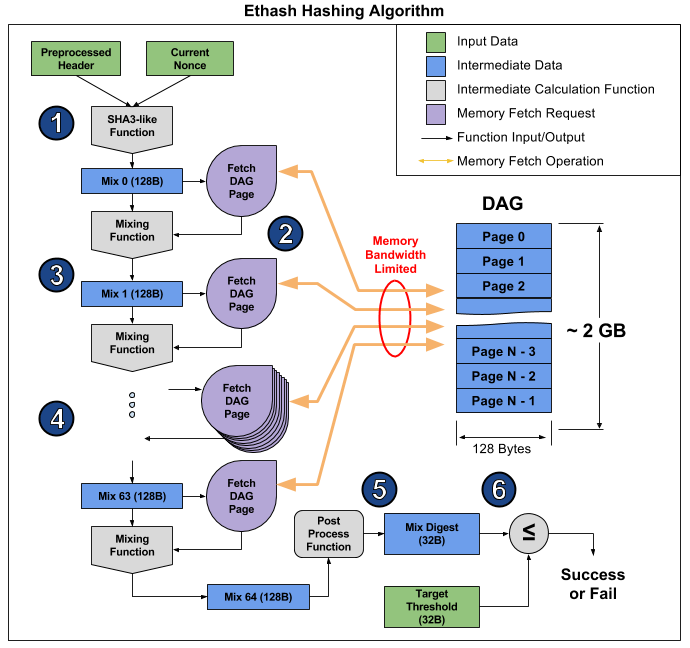
\includegraphics[width=250px,keepaspectratio]{ethash_algorithm.png}
\caption{\label{fig:ethash} Ethash}
\end{figure}

As time goes on, mining Ethereum becomes more and more difficult. The Proof-of-Work difficulty and total hashrate of the network has been steadily increasing over time, with the current difficulty at 1612.737TH and the respective hashrate at 109.138TH/s ~\cite{etherscan}. This reflects the design of mining one block approximately every 12 seconds. As for mining rewards, the reward for mining a block has gone from 5 Ether to 3 ether, though the difficulty has significantly decreased, both due to the Byzantium fork. Furthermore, the DAG used for the Ethereum network is now more than 2GB, causing many GPU miners with cards of 2GB of memory to suffer in terms of hashrate.

For a normal Ethereum miner to function, the current block headers and the DAG are required to even begin mining. As we simply cannot afford to transfer the entire DAG to the browser and store it in memory, we propose an an alternative approach addresses some of these concerns.

% \subsection{Choice of Crypto-currency}
% \trishita{We had this section in the project report, but I am not sure if we need this anymore, so I commented it out}
% In choosing crypto-currencies to mine, it was preferable to mine a larger, well known currency to ensure that the research would have real-world implications if adopted. Monero was the clear favorite, as it was created with the intent of providing no benefit over CPU mining. However, there has already been a web browser miner implemented for the Monero in the form of CoinHive~\cite{coinhive}, so any such efforts with Monero would not be novel. CoinHive also takes in a certain percentage of all currency generated and as such has kept their code closed sourced which meant that we could not easily extend or improve their current implementation as part of our research. In addition, many websites that utilize Coinhive have not informed users of their "stealing of computing power". This has drawn negative attention toward Coinhive to the extent that the code has been classified as malware and is automatically blocked by most firewalls and anti-viruses by default. Bitcoin was another option that we considered, however, there were two foreseeable problems with the crypto-currency that we felt would be insurmountable in our research timeline. First, ASIC technology has become the new norm for mining Bitcoin which would mean our web browser solution would hardly be able to compete. Second, the sheer popularity of Bitcoin means the mining is highly competitive in itself so our baseline threshold for seeing results would be too high for any reasonable amount of work. 

% In the end, we decided that Ethereum would be the most beneficial crypto-currency for a new web browser implementation of a miner. First of all, there is no existing web browser miner for Ethereum, so our implementation would have a certain novelty. In addition, Ethereum also allows developers to create private testnets to experiment with the network, which is a valuable asset to create a distributed network of miners. Another major benefit of Ethereum is that its smart contracts are Turing complete, meaning that the system can be used for a lot more than just sending or receiving currency. This could lead to a growing popularity of the crypto-currency in the coming years. Lastly, using Ethereum also leaves room for further exciting research, as will be discussed in a later section.

% \subsection*{Work Distribution}
% Trishita produced the \verb|JavaScript| implementation of the browser miner and the \verb|Python| test node with some help from Daniel. Dennis provided statistics and data for comparison to the browser miner in addition to setting up and managing the private testnet to perform operations on. All of the members participated in research and understanding of core Ethereum functions such as Ethash and how to mine via Ethereum.
 

% ~\dennis{https://github.com/ethereum/wiki/wiki/Ethash-Design-Rationale, should cite this so that they know that we are aware that compute from cache is designed to be inefficient, maybe add a diagram?)}

\section{Our Approach}
We propose a lazy-evaluation based approach to alleviate the network and memory requirements for mining ethereum in a distributed scenario on browsers. Specifically, as soon as each browser connects to the central node, the node sends it the current header of the block being mined and the Cache. Once the browser receives the Cache, it allocates an array buffer to store the DAG slices that will be computed in the future. (Note that the length of the buffer is a variable parameter that we experiment with in our analysis). Once this happens, the browser can start iterating over nonces to compute hashes.  

% The approach involves each browser allocating a fixed buffer to store the DAG, which is initially empty when the web page first loads. (Note that the size of this buffer is a parameter that can be adjusted depending on how much memory the client has.) The browser then starts mining, and 
Since, to begin with, the browser does not have any slices of the DAG, it must compute each slice on the fly using the Cache. However, for every such slice that the browser computes, it then stores it in the buffer (if it fits within the allocated bounds, otherwise it is simply discarded), for quicker access in the future. Hence, as time passes, the buffer starts filling up and so more and more slices are quickly accessed from the buffer rather than being computed from the ground-up, which makes hash computations faster with time. This has the effect that the longer the user remains on the web-page, the better the hashrate gets for that user. 
% If the allocated buffer is too small (as would be needed for some clients that do not have enough memory), and the computed slice cannot be fit in it, it is simply thrown away and again recomputed from the cache when needed.

% With respect to DAG lookups to compute each hash, the browser first checks if it already has the required slice in its buffer. If it does, it simply uses that, else it uses the Cache to compute that slice on the fly and then store it for future reference (if it fits in the buffer). Hence, initially the buffer starts out empty and so all DAG slices must be computed on the fly, and then stored in the buffer. However, 

\subsection{Information theoretic bounds}
With this lazy-evaluation based approach, we can calculate exactly how many hashes we would have to compute in order to fill up a buffer of a given size. This approach is a variation of the coupon collector problem \cite{couponCollector}. For our purposes, let us assume the following:
\begin{gather}
    Number\;of\;DAG\;slices = n\\
    Size\;of\;buffer\;as\;a\;fraction\;of\;the\;total DAG = i\;;i=[0,1]
\end{gather}
If we have buffered \verb|x| slices so far, the probability of obtaining a new slice is given by:
\begin{gather}
  P_x = \frac{ni-x}{n}
\end{gather}
The event of obtaining a new slice after having already collected \verb|x| out of the \verb|ni| slices that can be buffered can be modeled as a geometric distribution. Hence, the expected number of trials $t_x$ it takes to get a new  slice after having seen \verb|x| out of the \verb|i| slices is:
\begin{gather}
  E(t_x) = \frac{1}{P_x} = \frac{n}{ni-x}
\end{gather}
By linearity of expectation, the total number of trials it would take to see all \verb|x| slices is:
\begin{gather}
  E(t) = \sum_{x=0}^{ni-1}E(t_x)\\
    E(t) = \sum_{x=0}^{ni-1}P_x = \sum_{x=0}^{ni-1}\frac{n}{ni-x} = n\sum_{x=0}^{ni-1}\frac{1}{ni-x}
\end{gather}
Since the summation represents the harmonic series, the expected value can be approximated as follows:
\begin{gather}
  E(t) = n\log{ni}
\end{gather}
Now, equation ~\ref{eq:7} is in terms of the number of individual accesses of the DAG. In order to get the expected number of Hashes (as opposed to the expected number of individual DAG slice accesses), we need to divide by 64 since each hash involves 64 accesses of the DAG. Hence if we define: 
\begin{gather}
    Number\;of\;hashes\;computed = H
\end{gather}
\begin{gather}
  E(H) = \frac{n\log{ni}}{64}
\end{gather}
Now, let us do a simple calculation for one extreme case, where $i = 1$ (i.e., we allocate a buffer as large as the entire DAG on the browser), in order to get an upper bound on the number of hashes it would take to fill this buffer up. The private test network for Ethereum we used had a total of 16777186 slices in the DAG, which means it would take:
\begin{gather}
  E(H) = \frac{16777186*\log{16777186}}{64} = 4.36*10^6\;hashes
\end{gather}
Hence, it takes around 4 million hashes to fill up a buffer as large as the entire DAG. If $i < n$, the number of hashes should be less than 4 million. So effectively, 4 million hashes is a very lose upper bound on the number of hashes needed to fill up a DAG buffer.

Now let us say that we do not want to wait for the entire buffer to fill up -- how many hashes would we have to compute until a reasonable fraction of the buffer is full? Concretely speaking, let us assume the following:
\begin{gather}
  Fraction\;of\;DAG\;buffer\;to\;be\;filled = f;\;f \in [0,1]
\end{gather}
Then, for a buffer with space for \verb|i| slices, the number of slices we want to fill it with in order for a fraction \verb|f| of it to be full would be: 
\begin{gather}
  Number\;of\;slices\;to\;fill\;DAG\;buffer\;with = nfi
\end{gather}
This would modify equation \ref{eq:6} for the expected number of trials to fill up a fraction \verb|f| of the DAG buffer to be as follows:
\begin{gather}
    E(t) = \sum_{x=0}^{nfi}P_x = \sum_{i=0}^{nfi}\frac{n}{ni-x} = n\sum_{x=0}^{nfi}\frac{1}{ni-x}\\
    E(t) = n\sum_{x=0}^{nfi}\frac{1}{ni-x}
\end{gather}
This is essentially an early termination of the summation, and can be expressed as follows:
\begin{gather}
    E(t) = n\sum_{i=0}^{nfi}\frac{1}{ni-x} = n(\sum_{x=0}^{ni-1}\frac{1}{ni-x} - \sum_{x=nfi}^{ni-1}\frac{1}{ni-x})\\
    E(t) = n(\log{ni} - \log{(ni-nfi)}) \\
    E(t) = n\log{\frac{1}{1-f}}
\end{gather}
Again, we divide by 64 to obtain the expected number of hash computations:
\begin{gather}
    E(H) = \frac{n\log{\frac{1}{1-f}}}{64}
\end{gather}
Interestingly \verb|E(H)| does not depend on \verb|i|; the size of the DAG buffer as a fraction of the entire DAG. Figure X shows a graph of how \verb|E(H)| varies as a function of the fraction of the buffer that we want to be full, \verb|f| if we set $n = 16777186$ (the total number of DAG slices on the experimental private test network). 

From figure X we see that even computing merely 800,000 hashes fills our DAG buffer by more than 95\%! Beyond that, the marginal cost of computing more hashes outweighs the 
Finally, let us compute what the buffer hit rate should be for a given buffer size when the number of hashes computed tends to infinity. For this, let:
\begin{gather}
  Buffer\;hit\;rate = R \\
    Number\;of\;hashes\;computed = H
\end{gather}
Then,
\begin{gather}
  \lim_{H\to\infty}R = \frac{i}{n}
\end{gather}
This is because after a finite number of hashes, the buffer becomes full. Which means for any random slice of the DAG we pull out, the probability of it being in the buffer is $\frac{i}{n}$. However, the buffer hit rates were extremely low when H was close to 0 low $H\to\infty$

% We must also point out that in order to optimize the code for the specific cases, we have separate implementations for each of these two extreme edge cases. We also have another two separate implementations for the hybrid approach (where we store parts of the DAG and compute the other slices from the cache). The first hybrid implementation does not store the slices of the DAG the browser computes from the cache, while the second does (until it exhausts the storage space allocated to the DAG). The differences between each of the four implementations mainly lies in the data structures used to store the DAG, and is outlined follows:
% \begin{enumerate}
% \item Browser stores entire DAG in memory: We store the DAG in an array in order to get constant lookup times. The Cache is stored in an array of integers.
% \item Browser stores part of the DAG sent by the central node in memory and computes the other necessary slices from the Cache and stores these slices for future reference: Here, we need to store the DAG in a \verb|JavaScript| object (which is akin to a Hash Map). In this data structure, the keys correspond to the index of the DAG slice, and the value corresponds to the slice itself. We need a Hash Map as opposed to an array because we also store the slices that are generated on-the-fly from the Cache in this data structure. Since these slices are from random indices, we cannot store them at their correct indices in the array without allocating an array as large as the entire DAG itself -- which defeats the purpose of storing just a part of the DAG.
% \item Browser stores part of the DAG sent by the central node in memory and computes the other necessary slices from the Cache and \emph{does not} store these slices for future reference: Here, we just store the part of the DAG sent by the central server in memory, which we can compactly keep in an array since the central server sends consecutive slices.
% \item Browser stores none of the DAG and computes all the slices from the Cache: We do not store the DAG at all, but just the Cache in an array of integers.
% \end{enumerate}

\section{Architecture}
\begin{figure}[H]
\centering
\includegraphics[width=250px,keepaspectratio]{miningpool.png}
\caption{\label{fig:miningpool} Distributed Ethereum Mining}
\end{figure}

% A private Ethereum testnet is deployed to decrease the difficulty of mining so that the browsers clients can reliably mine at least some Ether. This can be easily ported to the real Ethereum network as we are using \verb|geth|, the Go implementation written for interacting with the Ethereum network. 
% The central Ethereum node is set up using \verb|geth|, which serves as the wallet that all the browser miners will point to.

Our architecture was centered around two client-side Ethereum miners written in \verb|JavaScript| and \verb|WebAssembly|. The central node that co-ordinates all workers (browsers) was an improvised version of \verb|geth| ~\cite{geth}, a real world Ethereum miner written in \verb|Go|. \verb|Geth| typically runs as a standalone miner that mines on the machine it is running. We modified it so that instead of mining all by itself, it simply sends over the necessary data needed to mine (the hash of the Block Header and the Cache) to any client that connects to it on port \verb|9000|. After recieving the necessary data, the browser allocates a buffer for the DAG in order to store future slices. Note that the buffer for the DAG is implemented an array of ints (with a DAG slice being 16 ints long), so as to make each lookup in the buffer $\theta(1)$. At this point, it can then begin to search for a solution. 

For our miner, we modeled our \verb|JavaScript| implementation based on the ~\verb|node.js| implementation of Ethash ~\cite{ethash}. To begin, the miner creates a random nonce and the computes the hash (using the Cache and the buffered DAG) as discussed in the previous section. It will continue to perform this action on new nonces until one of two scenarios occur; it finds a nonce such that the computed hash is below the given threshold or the process has timed out. In the former case, the browser submits the result back to the node and then asks the node for a new block header and the Cache. Otherwise if it has timed out without finding a result, the browser simply polls the node for the current block header and Cache . This process will continue until the user moves away from the website or closes their browser. 
We must point out that this time out is necessary since we want the browser to work with the most recent block header and Cache. The block header can become stale if that particular block has already been mined, and the Cache can become stale if the Ethereum network transitions into a new Epoch (happens once every 30,000 blocks). 
We must point out that both our current implementations in \verb|JavaScript| and \verb|WebAssembly| require no external dependencies, and therefore can be directly embedded into any website. For a diagramatic view our our design, see Figures~\ref{fig:hybridArchitecture}.

\begin{figure}[H]
\centering
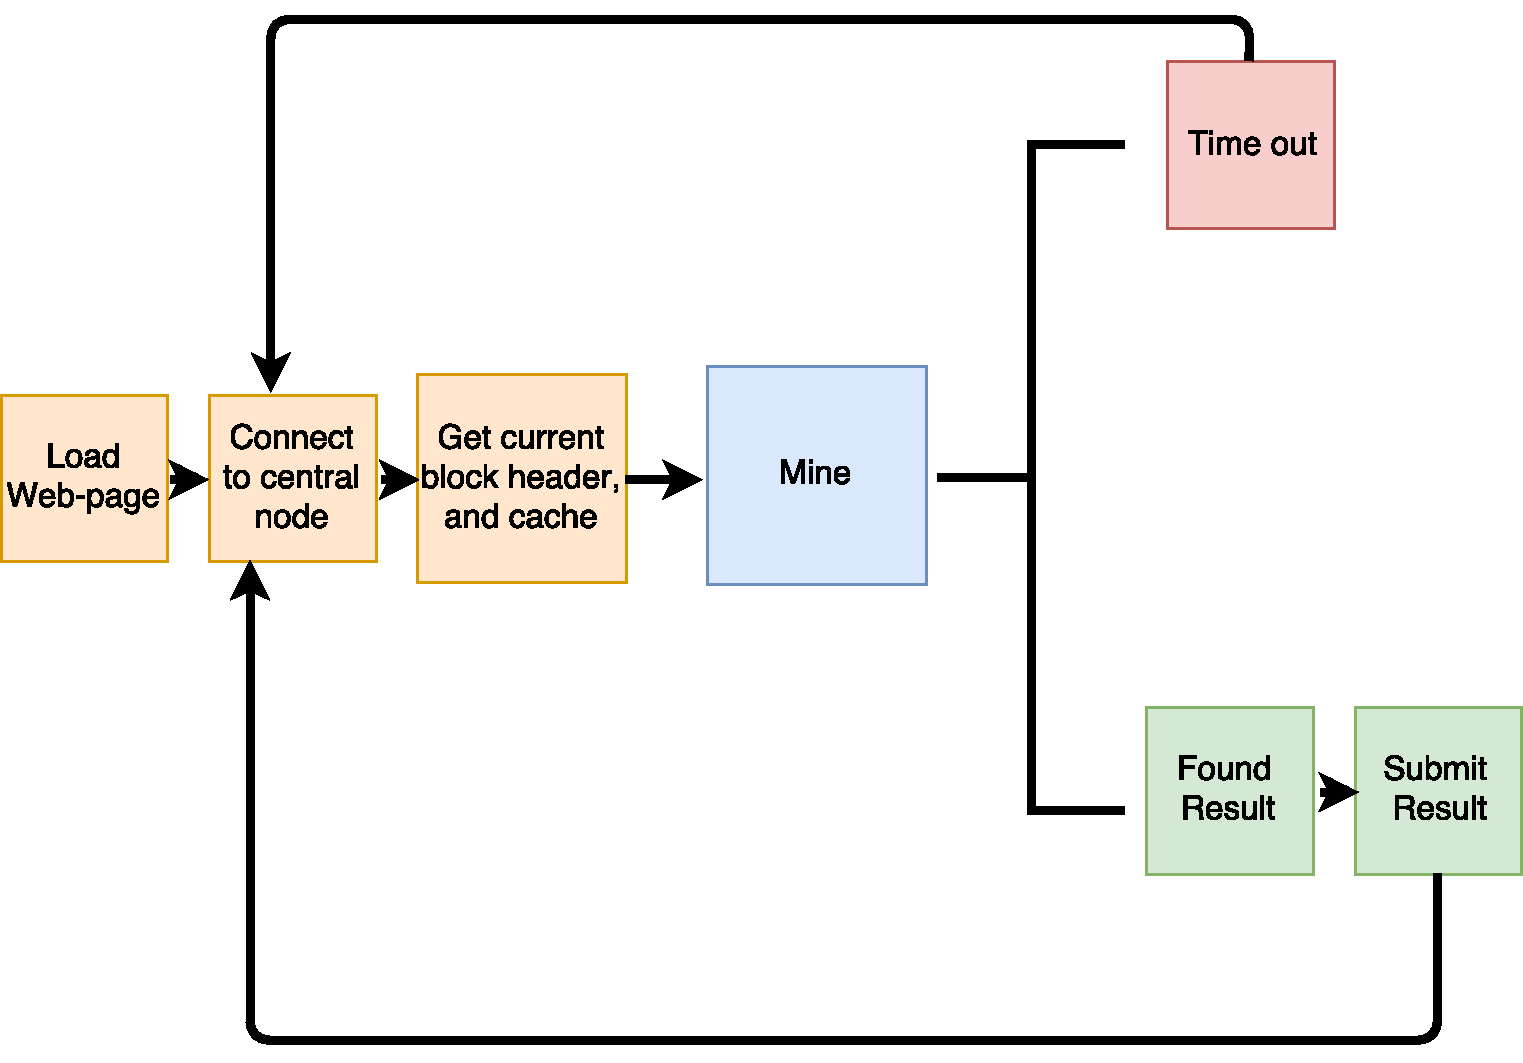
\includegraphics[width=250px,keepaspectratio]{Hybrid-Miner.pdf}
\caption{\label{fig:hybridArchitecture} Web Miner Architecture}
\end{figure}

% \section{Challenges}
% There were a multitude of challenges in creating such a distributed \verb|JavaScript| implementation of an Ethereum miner, we encountered a handful of challenges, some of which we were able to overcome and some that could be part of future work. One of the major decisions we needed to make was how to make sure the website would not become unresponsive due to a long running \verb|JavaScript| job. The reason this is an issue is because \verb|JavaScript| is a blocking language by nature, so if this job ran for too long no other \verb|JavaScript| responsible for website functionality could execute. As a workaround, we could schedule the hash computations to only run when the browser is idle using the \texttt{requestIdleCallback()} API. However, one must bear in mind that this would result in a lower hash rate and the API is not even supported in all browsers. 

% The other major challenges dealt with the DAG aspect of Ethereum. Even though we were able to limit the amount of the DAG sent to just the essential slices, these slices are still quite large to continuously be sent over the network. This leads to a lot of network bandwidth consumption.

%One of the more pertinent issues in mining Ethereum in such a fashion is how Ethereum operates. For starters, the Ethereum Proof-of-Work algorithm Ethash is designed to favor GPU mining rather than CPU mining, providing us with a innate handicap to work with. In addition, Ethash requires a 1GB DAG or Directed Acyclic Graph to be created and stored into memory for a machine to generate and verify hashes. Finally, in order to connect to the Ethereum network, a full Ethereum node must be set up to sync and add mined blocks to the blockchain. All of these issues considered, the processing power from a fraction of a CPU is wholly insufficient to profitably mine any amount of ether. Thus, distribution of computational work must be considered.

\section{Results}
\subsection{Experimental set up}
Our experimental set up consisted of a machine with an Intel i7-7700HQ processor with 4 cores and 16GB ram. These results were obtained from a private Ethereum test network at Epoch 0. The DAG size was 16777186 slices (with each slice being a sequence of 16 ints). The cache size was X.

\subsection{Baseline results}
For our control results, we ran \verb|Geth| ~\cite{geth}, a native miner written in \verb|Go| that stores the entire DAG in memory from the start (as opposed to using this lazy evaluation approach), and obtained an average hashrate of X H/s. We also ran our lazy-evaluation based miner written in C++ outside of the browser, and obtained the following results. 
Figure X below shows a heat-map of how the hash rate varies as a function of both the size of the buffer allocated to store the DAG (as a percentage of the size of the entire DAG) and the number of hashes computed in the browser. Figures X then shows a heat-map of how the DAG buffer hit-rate varies as a function of both the size of the buffer allocated to store the DAG and the number of hashes computed in the browser. 

% . Since the hashrate determines how fast a mining rig can verify a nonce, it was necessary to ensure that our results were not skewed due to the differences in computing power between computers. Using this machine, we recorded the hashrates for CPU performance and GPU performance on our private Ethereum testnet. 
% Additionally, we also recorded the hashrates for CPU mining in a Kali Linux VM. As we can see in the figure below, the GPU clearly outperforms the CPUs resulting in an average hashrate of 5.72MH/s. As for the CPUs, both miners performed about the same, both hovering around a respectable 210kH/s.
% \begin{figure}[H]
% \centering
% \includegraphics[width=250px,keepaspectratio]{GPU.png}
% \caption{\label{fig:gpu} GPU vs CPU Hashrates}
% \end{figure}

% \begin{figure}[H]
% \centering
% \includegraphics[width=250px,keepaspectratio]{CPU.png}
% \caption{\label{fig:cpu} VM CPU vs CPU Hashrates}
% \end{figure}

\subsection{Implementation Results}

% This happens because as described before, for the hybrid implementation where we store a small part of the DAG, we had to store the DAG in a \verb|javascript| object (Hash Map), with the ``keys'' being the index of the DAG and the value being the 512 bit slice that corresponds to that index. However, key-value look up times with \verb|JavaScript| objects are slow, according to the V8 design documentation for the language: ``Most JavaScript engines use a dictionary-like data structure as storage for object properties - each property access requires a dynamic lookup to resolve the property's location in memory. This approach makes accessing properties in JavaScript typically much slower than accessing instance variables in programming languages like Java and Smalltalk.'' ~\cite{AttrLookupLatency} This explains why storing larger and larger chunks of the DAG gives worse Hash rates, since it takes longer and longer to look up the required slices from the Hash Map. Indeed, this is why not storing the DAG at all, and just computing the slices from the Cache gives a high hash rate of \~ 1500 hashes/sec. The other extreme -- storing the entire DAG in memory is also slow because it takes up a lot of memory on the client's system. 

Note that this is the computational power of one machine and in reality, there would be hundreds or thousands of machines mining simultaneously, which will be analyzed in the next section. In comparison to Monero or Bitcoin browser miners who mine on an average of about 30-60H/s, our hashrate is significantly better than those.

\subsection{Difference Between Baseline and Implementation}
We see that the average hashrate outperforms 
% In a one to one comparison with CPU/GPU miners, the browser miner's hashrate is pitifully low. However, in theory, many machines would be accessing the site at the same time, significantly increasing the total computing power of the browser miner cluster. To calculate the results, we used a traffic analysis website ~\cite{traffic} to determine how many views and how long the average user stayed on the site in a span of six months. Using that data, we were able to calculate an estimated "visitors per second" that a site had. This, along with the hashrate of our browser miner, allowed us to estimate the total computing power of the cluster given a specific website. And as monetization is the objective, the cluster hashrate was plugged into an Ethereum profitability calculator~\cite{coinwarz} to examine how much would be earned. The results are shown in Figure ~\ref{fig:total}.
% \begin{figure}[H]
% \centering
% \includegraphics[width=250px,keepaspectratio]{Total.png}
% \caption{\label{fig:total} Calculated Estimated Hashrates}
% \end{figure}
% For analysis, we selected four websites indicating varying levels of website traffic, all with views more than 10 million per six months. Note that some of these websites (such as \verb|xkcd.com| and \verb|bu.edu|) do not normally have paid promotions for monetization and are only being used for an approximation on how much they would earn if they implemented our browser miner. As you can see, BU and \verb|xkcd.com| both did rather poorly in terms of annual income. However, the NY Times fared significantly better than a solo CPU miner, about 3 times better. Finally, Wikipedia topped all of them including the GPU miner with total annual earnings of \verb|$496.85|. Please also know that these income calculations do not include the cost of electricity as our implementation's energy consumption and cost depends on too many variables such as the way a specific browser handles calculations and the energy efficiency of each user's computer.

% \subsection{[New Results]}
% \subsubsection{Traditional Miner}
% As the DAG is incredibly large, attempts at a traditional miner operating on a browser became virtually impossible as the browser could not handle that much memory and ended up crashing.

% \subsubsection{Compute from Cache Miner}
% Just off of computing from the cache, our results seem promising. On average, computing DAG slices on demands from the cache yielded a hashrate of 127H/s. Theoretically, the miners that accessed from stored DAG slices would result in even higher hashrates.
% \begin{figure}[H]
% \centering
% \includegraphics[width=250px,keepaspectratio]{cache.PNG}
% \caption{\label{fig:total} Compute from Cache Miner}
% \end{figure}

% \subsubsection{Partial DAG + Cache Miner}
% However, contrary to our belief, having the DAG present in our test seemed to have slowed down the hashrate a bit. In addition, the hashrate appears to be relatively unaffected based on how many DAG slices were sent, despite the increasing usage of the slices provided to the client miner.
% \begin{figure}[H]
% \centering
% \includegraphics[width=250px,keepaspectratio]{partial.PNG}
% \caption{\label{fig:total} Partial DAG Sent, with Missing Slices Computed from Cache}
% \end{figure}

% \subsubsection{Partial DAG + Cache Miner /w Storage (Array)}
% This miner implementation used an array to store the DAG. It appears that by adding in the storage of slices, the performance did slightly improve. However, the performance remained unaffected by the changing quantity of DAG slices sent to the browser miner.
% \begin{figure}[H]
% \centering
% \includegraphics[width=250px,keepaspectratio]{partial_store_array.PNG}
% \caption{\label{fig:total} Partial DAG Sent, with Missing Slices Computed from Cache and Stored with Existing DAG slices}
% \end{figure}
% Also as seen before, the slices stored hit rate does go up the more slices are sent.
% \begin{figure}[H]
% \centering
% \includegraphics[width=250px,keepaspectratio]{partial_store_array_hitrate.PNG}
% \caption{\label{fig:total} Calculated Estimated Hashrates}
% \end{figure}

% \subsubsection{Partial DAG + Cache Miner w/ Storage (Hash Map)}
% Finally, instead of using an array to store the DAG, a Hash Map was used.This implementation provided the most biased results, as the data clearly indicates that the more DAG slices sent or cached in the Hash Map, the worse the miner's performance becomes. In addition, this miner performed the worst out of all of them, resulting in an incredibly low hash rate in comparison to just computing from the cache.
% \begin{figure}[H]
% \centering
% \includegraphics[width=250px,keepaspectratio]{partial_store_hashmap.PNG}
% \caption{\label{fig:total} Partial DAG Sent, with Missing Slices Computed from Cache and Stored with Existing DAG slices}
% \end{figure}

% \subsection{Additional Notes}
% Note that all of these results came from a private Ethereum testnet and thus do not accurately reflect mining capabilities on the actual Ethereum Network. GPU mining should be on an order of magnitude faster in terms of hashrate as opposed to CPUs. Additional research may be necessary to see how browser mining pools remain profitable without sufficient hashrates to support them.

\section{Future Work}

While we were able to create a browser based miner for Ethereum, there is still work to be done. As was shown, our current implementation is far slower than the traditional methods for mining. A first step is to pinpoint the exact cause for such a slow hash rate. One way we can look to speed this process up is to tap into the client machine's GPU. There is a \verb|JavaScript| library called WebCL that binds to the OpenCL library which allows the \verb|JavaScript| to speak directly to the GPU for better parallel performance. Knowing that Ethereum was created for GPU mining and based on our results, it should provide a substantial improvement. In addition, because of the memory hard requirements of the Ethereum protocol we should also see a better performance if we can somehow get the DAG to be directly accessible to the client instead of having to send slices over the network to all the clients. Therefore, we want to look into the use of \verb|remoteStorage| ~\cite{remote}, which allows the user to have complete control over the data. By moving the data closer to the computation we are hoping to cut the added time caused by the network.

Ethereum is also currently working on Casper, their Proof-of-Stake algorithm, which has already been deployed to private testnets for testing. Working with that and the fact that the entire Casper code is available online, it would be possible to create a theoretical Proof-of-Stake distributed browser miner implementation in preparation for the fork. However, seeing as though Proof-of-Stake would virtually eliminate the necessity of massive amounts of processing power, users would most likely have to provide ``stakes" in order for such an implementation to be possible ~\cite{PoSproof}. Further research will be necessary to determine whether browser mining for Casper is viable or not, as the final form of Casper is still hazy and exactly how much "stake" is required to mine is uncertain.

%While the roadblocks of this project cause a viable solution for Ethereum browser mining to be almost unfeasible, the changes coming to Ethereum in the near future may prove otherwise. Since Proof-of-Work discourages miners over time due to reduction of rewards from mining, Ethereum will soon be moving to Proof-of-Stake via their algorithm Casper. With the introduction of Casper, mining will be less computationally intensive and require users to provide a "stake" in Ethereum in order to mine. Although it would require users to put in actual money to assist in obtaining stakes, this may prove for the better as users lose significantly less processing (the main computation would jsut come from verifying blocks as opposed to mining them). And provided that interest and infrastructure for Ethereum grows, people may probably already have "stakes" in Ethereum and thus would not be as opposed to adding that to a pool.


% An example of a floating figure using the graphicx package.
% Note that \label must occur AFTER (or within) \caption.
% For figures, \caption should occur after the \includegraphics.
% Note that IEEEtran v1.7 and later has special internal code that
% is designed to preserve the operation of \label within \caption
% even when the captionsoff option is in effect. However, because
% of issues like this, it may be the safest practice to put all your
% \label just after \caption rather than within \caption{}.
%
% Reminder: the "draftcls" or "draftclsnofoot", not "draft", class
% option should be used if it is desired that the figures are to be
% displayed while in draft mode.
%
%\begin{figure}[!t]
%\centering
%\includegraphics[width=2.5in]{myfigure}
% where an .eps filename suffix will be assumed under latex, 
% and a .pdf suffix will be assumed for pdflatex; or what has been declared
% via \DeclareGraphicsExtensions.
%\caption{Simulation Results}
%\label{fig_sim}
%\end{figure}

% Note that IEEE typically puts floats only at the top, even when this
% results in a large percentage of a column being occupied by floats.


% An example of a double column floating figure using two subfigures.
% (The subfig.sty package must be loaded for this to work.)
% The subfigure \label commands are set within each subfloat command, the
% \label for the overall figure must come after \caption.
% \hfil must be used as a separator to get equal spacing.
% The subfigure.sty package works much the same way, except \subfigure is
% used instead of \subfloat.
%
%\begin{figure*}[!t]
%\centerline{\subfloat[Case I]\includegraphics[width=2.5in]{subfigcase1}%
%\label{fig_first_case}}
%\hfil
%\subfloat[Case II]{\includegraphics[width=2.5in]{subfigcase2}%
%\label{fig_second_case}}}
%\caption{Simulation results}
%\label{fig_sim}
%\end{figure*}
%
% Note that often IEEE papers with subfigures do not employ subfigure
% captions (using the optional argument to \subfloat), but instead will
% reference/describe all of them (a), (b), etc., within the main caption.


% An example of a floating table. Note that, for IEEE style tables, the 
% \caption command should come BEFORE the table. Table text will default to
% \footnotesize as IEEE normally uses this smaller font for tables.
% The \label must come after \caption as always.
%
%\begin{table}[!t]
%% increase table row spacing, adjust to taste
%\renewcommand{\arraystretch}{1.3}
% if using array.sty, it might be a good idea to tweak the value of
% \extrarowheight as needed to properly center the text within the cells
%\caption{An Example of a Table}
%\label{table_example}
%\centering
%% Some packages, such as MDW tools, offer better commands for making tables
%% than the plain LaTeX2e tabular which is used here.
%\begin{tabular}{|c||c|}
%\hline
%One & Two\\
%\hline
%Three & Four\\
%\hline
%\end{tabular}
%\end{table}


% Note that IEEE does not put floats in the very first column - or typically
% anywhere on the first page for that matter. Also, in-text middle ("here")
% positioning is not used. Most IEEE journals/conferences use top floats
% exclusively. Note that, LaTeX2e, unlike IEEE journals/conferences, places
% footnotes above bottom floats. This can be corrected via the \fnbelowfloat
% command of the stfloats package.

\section{Conclusion}
We have successfully created a proof of concept distributed, web-based Ethereum miner that can be used towards monetizing electronic content. Our implementation is standalone, and hence can simply be embedded within a website without having the client install any external dependencies. Furthermore, we provide an API that can be used by any implementation of Ethereum (\verb|geth| or Ethereum's implementation in \verb|C++|). We believe this can be a be especially viable in a private testnet, within a company for example, and with further research has the potential to make a real impact.

% conference papers do not normally have an appendix


% % use section* for acknowledgement
% \section*{Acknowledgment}

% trigger a \newpage just before the given reference
% number - used to balance the columns on the last page
% adjust value as needed - may need to be readjusted if
% the document is modified later
%\IEEEtriggeratref{8}
% The "triggered" command can be changed if desired:
%\IEEEtriggercmd{\enlargethispage{-5in}}

% references section

% can use a bibliography generated by BibTeX as a .bbl file
% BibTeX documentation can be easily obtained at:
% http://www.ctan.org/tex-archive/biblio/bibtex/contrib/doc/
% The IEEEtran BibTeX style support page is at:
% http://www.michaelshell.org/tex/ieeetran/bibtex/
%\bibliographystyle{IEEEtran}
% argument is your BibTeX string definitions and bibliography database(s)
%\bibliography{IEEEabrv,../bib/paper}
%
% <OR> manually copy in the resultant .bbl file
% set second argument of \begin to the number of references
% (used to reserve space for the reference number labels box)
\begin{thebibliography}{1}
\bibitem{Adblock} Gundlach, Micheal. AdBlock browser extension. AdBlock. Software, 2009.

\bibitem{ethash}Matthew Wampler, et al. Ethash. Computer software. GitHub. Vers. 23.1. GitHub, 11 Jan. 2015. Web. 24 Feb. 2018. <https://github.com/ethereum/ethash>. 

\bibitem{BraveBrowser} Eich, Brendan and Brian Bondy. Brave Browser. Brave Software. Software, 2015.

\bibitem{decliningRevenue} Hern, Alex. “Adblock Plus: the Tiny Plugin Threatening the Internet's Business Model.” The Guardian, Guardian News and Media, 14 Oct. 2013, www.theguardian.com/technology/2013/oct/14/the-tiny-german-company-threatening-the-internets-business-model.

\bibitem{dagger-hashimoto} Buterin, Vitalik, et al. “Ethereum/Wiki.” GitHub, GitHub, 9 Feb. 2014, github.com/ethereum/wiki/blob/master/Dagger-Hashimoto.md. 

\bibitem{noSubscriptions} Rosenwald, Micheal. “Digital News Consumers Unlikely to Pay for Content and Increasingly Block Ads.” Columbia Journalism Review, Columbia Journalism Review, 15 June 2015, www.cjr.org/analysis/reuters\_digital\_news\_report.php.

\bibitem{payPerClick} Fessenden, Therese. “Nielsen Norman Group.” The Most Hated Online Advertising Techniques, Nielsen Norman Group, 4 June 2017, www.nngroup.com/articles/most-hated-advertising-techniques/.

\bibitem{celebEndorse} Awad, Amal. “A Study in Scarlett: The Ethics of Celebrity Endorsement.” – Opinion – ABC Religion \&Amp; Ethics (Australian Broadcasting Corporation), Amal Awad ABC Religion and Ethics, 30 Jan. 2014, www.abc.net.au/religion/articles/2014/01/31/3935443.htm.

% \bibitem{Boldrin} Boldrin, F., et al. “Distributed Computing Through Web Browser.” Distributed Computing Through Web Browser - IEEE Conference Publication, University of Ferrara, ieeexplore.ieee.org/document/4350073/.

\bibitem{scheduling}
Ramamritham, Krithi, and John A. Stankovic. "Dynamic task scheduling in hard real-time distributed systems." IEEE software 1.3 (1984): 65.

\bibitem{parallel}
Shirazi, Behrooz A., Krishna M. Kavi, and Ali R. Hurson. Scheduling and load balancing in parallel and distributed systems. IEEE Computer Society Press, 1995.

\bibitem{orca}
Bal, Henri E., M. Frans Kaashoek, and Andrew S. Tanenbaum. "Orca: A language for parallel programming of distributed systems." IEEE transactions on software engineering 18.3 (1992): 190-205.

\bibitem{WebFlow}
Bhatia, Dimple; Burzevski, Vanco; Camuseva, Maja; and Fox, Geoffrey C., "WebFlow - A Visual Programming Paradigm for Web/Java Based Coarse Grain Distributed Computing" (1997).
Northeast Parallel Architecture Center.

\bibitem{Cushing} Cushing, Reginald, et al. “Distributed Computing on an Ensemble of Browsers.” IEEE Internet Computing, IEEE, 1 Sept. 2013, www.computer.org/csdl/mags/ic/2013/05/mic2013050054.html.

\bibitem{randmemohash} Lerner, Sergio Demian. "STRICT MEMORY HARD HASHING FUNCTIONS (PRELIMINARY V0. 3, 01-19-14)."

\bibitem{coinhive}
The Coinhive Team. Coinhive browser extension. Coinhive. Software, 2017.

\bibitem{pow}
Laurie, Ben, and Richard Clayton. "Proof-of-work proves not to work; version 0.2." Workshop on Economics and Information, Security. 2004.

\bibitem{casper}
Hertig, Alyssa. “Ethereum's Big Switch: The New Roadmap to Proof-of-Stake.” CoinDesk, CoinDesk, 16 May 2017, www.coindesk.com/ethereums-big-switch-the-new-roadmap-to-proof-of-stake/. 

\bibitem{pos}
Dmitry Buterin, et al. “Proof of Work vs Proof of Stake: Basic Mining Guide.” Blockgeeks, Blockgeeks, 24 July 2017, blockgeeks.com/guides/proof-of-work-vs-proof-of-stake/. 

\bibitem{arc}
The ArcticCoin Team. ArcticCoin crypto-currency. ArcticCoin. Software, 2015.

\bibitem{Monero} “Monero - Secure, Private, Untraceable.” Getmonero.org, The Monero Project, getmonero.org/.

\bibitem{Duda} Duda, Jerzy, and Wojciech Dłubacz. “Distributed Evolutionary Computing System Based on Web Browsers with Javascript.” ACM Digital Library, Springer-Verlag, dl.acm.org/citation.cfm?id=2451764.2451780.

\bibitem{traffic} The SimilarWeb Team. SimilarWeb LTD 2017. (https://www.similarweb.com/)

\bibitem{coinwarz}Coinwarz Ethereum Mining Calculator and Profit Calculator. Coinwarz 2017. (https://www.coinwarz.com/calculators/ethereum-mining-calculator)

\bibitem{PoSproof}Dale, Oliver. "Beginner's Guide to Ethereum Casper Hardfork: What You Need to Know". Blocknomi, 7 November 2017. (https://blockonomi.com/ethereum-casper/)

\bibitem{Ethmining}
Wood, Gavin. "Ethereum: A secure decentralised generalised transaction ledger." Ethereum Project Yellow Paper 151 (2014): 1-32.

\bibitem{geth}Péter Szilágyi, et al. Geth. Computer software. GitHub. Vers. 1.8.1. GitHub, 22 Dec. 2013. Web. 24 Feb. 2018. <https://github.com/ethereum/go-ethereum>. 

\bibitem{etherscan}Etherscan The Ethereum Block Explorer. Etherscan 2017. (https://etherscan.io/charts)

\bibitem{remote} remoteStorage: An open protocol for per-user storage on the Web. (https://remotestorage.io/)
\end{thebibliography}

\addtolength{\textheight}{-7cm}
\balance


% that's all folks
\end{document}